\documentclass[../../main.tex]{subfiles}
\graphicspath{{../../image/}{../../figure/}}
\begin{document}

\section{一般严格双曲方程组}\label{section:ch09-一般严格双曲方程组}

我们的下一个任务是:对特征族既不真正非线性、也不线性退化的方程组,描述容许波扇并构造相应的波曲线。此时 Lax $E$ 条件不再充分,无法筛选出 Riemann 问题的唯一解,因而要在激波上施加更强的 Liu $E$ 条件。

我们从标量守恒律\eqref{align:ch07-标量守恒律}入手,其中 $f(u)$ 可能有拐点。Liu $E$ 条件在此即 Oleinik $E$ 条件\eqref{align:ch08-oleinik}。由\cref{theorem:ch09-波扇结构}, Riemann 问题的解由两个常值状态 $u_{L}$ 与 $u_{R}$ 组成,二者由一个波连接,该波是一串激波和/或中心稀疏波。存在唯一一个这样的波,其激波满足 Oleinik $E$ 条件,它由如下程序构造:当 $u_{L}<u_{R}$(或 $u_{L}>u_{R}$)时,令 $g$ 为 $f$ 在区间 $[u_{L},u_{R}]$(或 $[u_{R},u_{L}]$)上的\emph{凸包}(或\emph{凹包});即 $g(u)$ 是所有凸组合 $\theta_{1}f(u_{1})+\theta_{2}f(u_{2})$(其中 $\theta_{1}\geqslant0$, $\theta_{2}\geqslant0$, $\theta_{1}+\theta_{2}=1$, $u_{1},u_{2}\in[u_{L},u_{R}]$(或 $[u_{R},u_{L}]$),且 $\theta_{1}u_{1}+\theta_{2}u_{2}=u$)的下确界(或上确界)。因而 $g$ 的图像可想象为:一条柔性弦,锚定于点 $(u_{L},f(u_{L}))$、$(u_{R},f(u_{R}))$,在障碍 $\{(u,v):u_{L}\leqslant u\leqslant u_{R},\ v\geqslant f(u)\}$(或 $\{(u,v):u_{R}\leqslant u\leqslant u_{L},\ v\leqslant f(u)\}$)之下(或之上)张紧。斜率 $\xi=g'(u)$ 是连续非减(或非增)函数,其逆 $u=\omega(\xi)$ 生成(一般为复合)波 $u=\omega(x/t)$。特别地, $g'(u)$ 的平直段产生激波,而 $g'(u)$ 严格单调的区间生成稀疏波。\cref{figure:ch09-标量复合波}描绘了一个例子,所得波由一个中心稀疏波、继之以一个接触间断、再继之以另一个中心稀疏波组成,后者右侧以一个左接触间断为界。

\begin{figure}[ht]
\centering
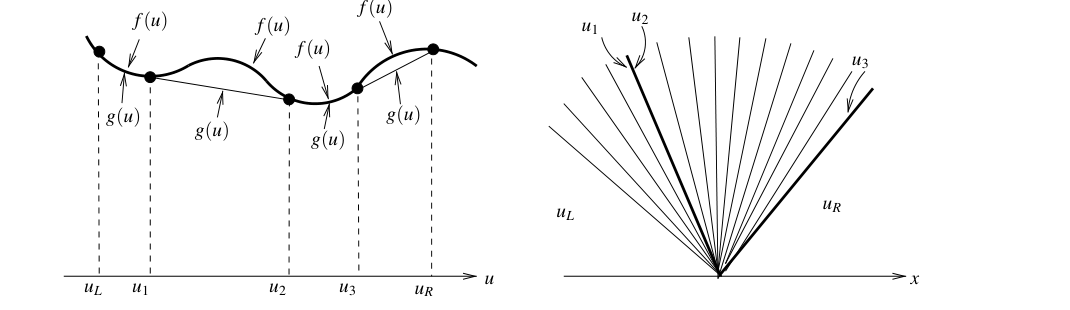
\includegraphics[width=0.85\textwidth]{ch09-fig05-01.png}
\caption{(左)凸包 $g$ 及其导出函数 $g'$;$g$ 的平直段对应激波。(右)相应的 $x$-$t$ 平面波扇,常值状态 $u_{L},u_{1},u_{2},u_{3},u_{R}$。}
\label{figure:ch09-标量复合波}
\end{figure}

为给研究一般方程组做准备,我们对\eqref{align:ch07-p系统}这一简单方程组构造波及相应波曲线,其中 $\sigma(u)$ 可能有拐点。此处 Liu $E$ 条件化为 Wendroff $E$ 条件\eqref{align:ch08-wendroff}。与真正非线性情形一样,我们取 $u$ 为参数,通过状态 $(\bar{u},\bar{v})$ 确定前向 $1$-波曲线 $\Phi_{1}$ 与后向 $2$-波曲线 $\Psi_{2}$,分别形如 $v=\varphi(u;\bar{u},\bar{v})$ 与 $v=\psi(u;\bar{u},\bar{v})$。回顾 Hugoniot 轨迹的方程\eqref{align:ch08-rdr}、稀疏波曲线的方程\eqref{align:ch07-p系统稀疏波}以及\eqref{align:ch08-wendroff},易验证
\begin{align}
\varphi(u;\bar{u},\bar{v})=\bar{v}+\int_{\bar{u}}^{u}\sqrt{g'(\omega;u,\bar{u})}\,\mathrm{d}\omega,
\label{align:ch09-9-5-1}
\end{align}
\begin{align}
\psi(u;\bar{u},\bar{v})=\bar{v}-\int_{\bar{u}}^{u}\sqrt{g'(\omega;u,\bar{u})}\,\mathrm{d}\omega,
\label{align:ch09-9-5-2}
\end{align}
其中 $g'(\omega;u,\bar{u})$ 是单调递增、连续可微函数 $g(\omega;u,\bar{u})$ 对 $\omega$ 的导数,该函数由如下程序构造:固定 $u\leqslant\bar{u}$(或 $u\geqslant\bar{u}$)时, $g(\cdot,u,\bar{u})$ 是 $\sigma(\cdot)$ 在区间 $[u,\bar{u}]$(或 $[\bar{u},u]$)上的凸包(或凹包)。事实上,与上面讨论的标量守恒律情形一样,状态 $(\bar{u},\bar{v})$ 与 $(u,v)$,其中 $v=\phi(u;\bar{u},\bar{v})$,由一个(一般为复合)$1$-波 $(\omega(x/t),v(x/t))$ 连接,其中 $\omega(\xi)$ 是函数 $\xi=\sqrt{g'(\omega;u,\bar{u})}$ 的逆,且
\begin{align}
v(\xi)=\bar{v}+\int_{\bar{u}}^{\omega(\xi)}\sqrt{g'(\omega;u,\bar{u})}\,\mathrm{d}\omega.
\label{align:ch09-9-5-3}
\end{align}

同样, $g'$ 的平直段产生激波,而 $g'$ 严格单调的区间生成稀疏波。在真正非线性情形 $\sigma''(u)<0$ 下,\eqref{align:ch09-9-5-1}与\eqref{align:ch09-9-5-2}退化为\eqref{align:ch09-9-4-1}与\eqref{align:ch09-9-4-2}。一旦 $\phi$ 与 $\psi$ 确定,Riemann 问题即可像真正非线性情形那样容易求解:通过方程\eqref{align:ch09-9-4-3}定位中间常值状态 $(u_{M},v_{M})$。

做完这一准备后,我们继续 somewhat 概略、非正式地描述一般方程组波曲线的构造。为避免各种退化所诱发的复杂纠缠,我们把研究限制在\emph{分段真正非线性}的 $i$-特征族上,其含义是:若 $U$ 是线性退化状态,即 $\mathrm{D}\lambda_{i}(U)R_{i}(U)=0$,则 $\mathrm{D}(\mathrm{D}\lambda_{i}(U)R_{i}(U))R_{i}(U)\neq0$。这特别蕴含:第 $i$ 特征族的线性退化状态集局部为余维数 $1$ 的光滑流形,且横截于向量场 $R_{i}$。标量守恒律\cref{lemma:ch08-激波速度符号}与等熵弹性方程组\cref{lemma:ch08-激波速度符号}满足此假设: $f(u)$ 与 $\sigma(u)$ 有孤立、非退化的拐点,即 $f'''(u)$ 与 $\sigma'''(u)$ 在 $f''(u)$ 与 $\sigma''(u)$ 为零的点处非零。即使做了这些简化,构造仍很复杂。若读者回头参照模型方程组\cref{lemma:ch08-激波速度符号}以说明每一步,思路会更清晰。熟悉\cref{lemma:ch08-激波速度符号}及其后评述也会有帮助。

假定第 $i$ 特征族分段真正非线性,我们考虑过一个真正非线性点 $\bar{U}$ 的前向 $i$-波曲线 $\Phi_{i}(\tau;\bar{U})$,不妨设 $\mathrm{D}\lambda_{i}(\bar{U})R_{i}(\bar{U})=1$。则 $\Phi_{i}$ 在真正非线性情形那样起步: $\tau$ 小且正时它与过 $\bar{U}$ 的 $i$-稀疏波曲线 $V_{i}(\tau;\bar{U})$ 重合;而 $\tau$ 负且接近零时它与过 $\bar{U}$ 的 $i$-激波曲线 $W_{i}(\tau;\bar{U})$ 重合。特别地,\eqref{align:ch09-9-3-7}成立。我们沿 $\tau$ 正向追踪 $\Phi_{i}$; $\tau<0$ 的描述完全类似。

对 $\tau>0$,只要 $V_{i}(\tau;\bar{U})$ 处于真正非线性区域 $\mathrm{D}\lambda_{i}(V_{i})R_{i}(V_{i})>0$ 内, $\Phi_{i}(\tau;\bar{U})$ 就一直沿 $i$-稀疏波曲线 $V_{i}(\tau;\bar{U})$ 走。现设 $V_{i}(\tau;\bar{U})$ 首次在状态 $\tilde{U}=V_{i}(\tilde{\tau};\bar{U})$ 处遇到第 $i$ 特征族的线性退化状态集: $\mathrm{D}\lambda_{i}(\tilde{U})R_{i}(\tilde{U})=0$。$\tilde{U}$ 附近的线性退化状态集构成余维数 $1$ 的流形 $\mathscr{M}$,横截于向量场 $R_{i}$;见\cref{figure:ch09-波曲线构造}(a,b)。

$\Phi_{i}$ 越过 $\tilde{U}$ 的延拓构造如下:取 $\tau^{*}<\tilde{\tau}$,且 $\tilde{\tau}-\tau^{*}$ 小,过状态 $U^{*}=V_{i}(\tau^{*};\bar{U})$ 画 $i$-激波曲线 $W_{i}(\zeta;U^{*})$。由\cref{lemma:ch08-激波速度符号}, $s_{i}(0;U^{*})=\lambda_{i}(U^{*})$;又因 $\mathrm{D}\lambda_{i}(U^{*})R_{i}(U^{*})>0$,\cref{lemma:ch08-激波速度符号}推出:对负 $\zeta$、接近 $0$ 时, $\dot{s}_{i}(\zeta;U^{*})>0$ 且 $s_{i}(\zeta;U^{*})<\lambda_{i}(W_{i}(\zeta;U^{*}))$。然而,穿过 $\mathscr{M}$ 后, $W_{i}(\zeta;U^{*})$ 进入 $\mathrm{D}\lambda_{i}(U)R_{i}(U)<0$ 的区域,从而 $\lambda_{i}(W_{i}(\zeta;U^{*}))$ 开始下降。最终达到 $\zeta^{*}$ 使 $s_{i}(\zeta^{*};U^{*})=\lambda_{i}(W_{i}(\zeta^{*};U^{*}))$。对 $\zeta<\zeta^{*}$,由\cref{lemma:ch08-激波速度符号},有 $s_{i}(\zeta,U^{*})>\lambda_{i}(W_{i}(\zeta;U^{*}))$ 且 $\dot{s}_{i}(\zeta,U^{*})<0$。最终达到值 $\zeta^{\sharp}$ 使 $s_{i}(\zeta^{\sharp};U^{*})=\lambda_{i}(U^{*})$。于是状态 $U^{\sharp}=W_{i}(\zeta^{\sharp};U^{*})$ 在右,与在左的 $U^{*}$ 由一个速度为 $\lambda_{i}(U^{*})$ 的左 $i$-接触间断连接。此激波满足 Liu $E$ 条件,因为对 $\zeta<\zeta^{\sharp}$, $s_{i}(\zeta;U^{*})>\lambda_{i}(U^{*})=s_{i}(\zeta^{\sharp};U^{*})>\lambda_{i}(U^{\sharp})$。因而,在左的 $\tilde{U}$ 与在右的 $U^{\sharp}$ 由一个容许 $i$-波连接,该波由连接 $U^{*}$ 到 $\tilde{U}$ 的 $i$-稀疏波与连接 $U^{\sharp}$ 到 $U^{*}$ 的容许左 $i$-接触间断组成。可以证明:当 $U^{*}$ 沿曲线 $V_{i}(\tau;\bar{U})$ 从 $\tilde{U}$ 向 $\bar{U}$ 移动时,相应的 $U^{\sharp}$ 描出一条曲线 $\Gamma$。若 $U^{*}=\tilde{U}$,则 $U^{\sharp}=\tilde{U}$,故 $\Gamma$ 在 $\tilde{U}$ 处从 $\tilde{U}$ 出发。此外, $\Gamma$ 在 $\tilde{U}$ 处与 $R_{i}(\tilde{U})$ 相切。我们把它接在 $V_{i}(\tau;\bar{U})$ 上,并据此以适当参数化把 $\Phi_{i}(\tau;\bar{U})$ 延拓到 $\tilde{U}$ 之外。

$\Phi_{i}(\tau;\bar{U})$ 将沿 $\Gamma$ 一直走到达到状态 $\hat{U}$,在那里下述两个可能首先出现之一发生:

\begin{figure}[ht]
\centering
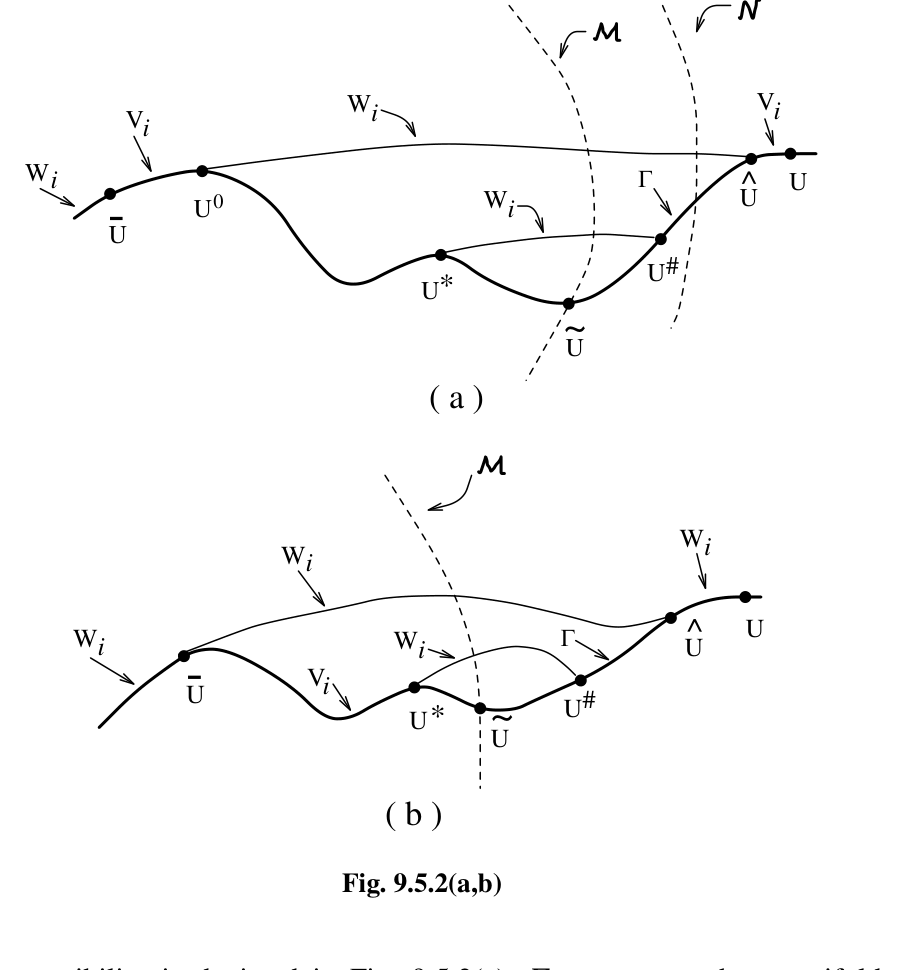
\includegraphics[width=0.7\textwidth]{ch09-fig05-02.png}
\caption{分段真正非线性方程组前向 $i$-波曲线的构造。(a) $\Gamma$ 穿过另一个线性退化流形 $\mathscr{N}$, $U^{*}$ 退回到 $U^{0}$;(b) $U^{*}$ 一路退到 $\tilde{U}$。}
\label{figure:ch09-波曲线构造}
\end{figure}

一种可能如\cref{figure:ch09-波曲线构造}(a)所示: $\Gamma$ 穿过第 $i$ 特征族的另一个线性退化状态流形 $\mathscr{N}$,进入 $\mathrm{D}\lambda_{i}(U)R_{i}(U)>0$ 的区域,最终 $U^{*}$ 退回到位置 $U^{0}$,使得相应的 $U^{\sharp}$(记作 $\hat{U}$)满足 $\lambda_{i}(\hat{U})=\lambda_{i}(U^{0})$。此时 $\Phi_{i}(\tau;\bar{U})$ 作为过 $\hat{U}$ 的 $i$-稀疏波曲线 $V_{i}(\zeta;\hat{U})$ 适当重新参数化后延拓到 $\hat{U}$ 之外。该曲线上任一状态 $U$ 在右与 $\bar{U}$ 由一个复合 $i$-波连接,该波由连接 $U^{0}$ 到 $\bar{U}$ 的 $i$-稀疏波、连接 $\hat{U}$ 到 $U^{0}$ 的 $i$-接触间断,以及连接 $U$ 到 $\hat{U}$ 的第二个 $i$-稀疏波组成。

另一种可能如\cref{figure:ch09-波曲线构造}(b)所示: $U^{*}$ 一路退回到 $\tilde{U}$,相应的 $U^{\sharp}$(记作 $\hat{U}$)满足 $\lambda_{i}(\hat{U})<\lambda_{i}(\bar{U})$。此时 $\hat{U}$ 落在过 $\bar{U}$ 的 $i$-激波曲线上,即 $\hat{U}=W_{i}(\hat{\tau};\bar{U})$。由于 $s_{i}(\hat{\tau};\bar{U})=\lambda_{i}(\bar{U})>\lambda_{i}(\hat{U})$,\cref{lemma:ch08-激波速度符号}推出 $\dot{s}_{i}(\hat{\tau};\bar{U})<0$。于是 $\Phi_{i}(\tau;\bar{U})$ 沿 $i$-激波曲线 $W_{i}(\tau;\bar{U})$ 延拓到 $\hat{U}$ 之外。该弧上任一状态 $U$ 在右与 $\bar{U}$ 由单个满足 Liu $E$ 条件的 $i$-激波连接。

通过继续这一程序,我们完成 $\Phi_{i}(\tau;\bar{U})$ 在中等强度波范围内的构造,对某些方程组甚至可用于强波。此外,仔细复查构造可验证: $\Phi_{i}$ 的图像包含了 $\bar{U}$ 充分小邻域中一切可由容许 $i$-波连接到 $\bar{U}$ 的状态。

如我们先前所见,在穿过任何线性退化状态流形之前, $\Phi_{i}$ 是 $C^{2,1}$ 的。第一次与这类流形相交后,其正则性可能降为 $C^{1,1}$;第二次相交之后可能变为仅 Lipschitz(参考文献见\cref{section:ch09-注记})。尽管如此,\eqref{align:ch09-9-3-2}仍成立,在中等强度波范围内,使 $P_{i}(\tau;U)$ 的 Lipschitz 常数变小的 $\tau$ 范围跨线性退化状态流形,且不依赖于其个数。因而,对任一严格双曲方程组,只要其通量可实现为一列分段真正非线性方程组通量的 $C^{1}$ 极限,即可追踪其波曲线。

后文\cref{section:ch09-粘性波扇}中将遇到一般严格双曲方程组波曲线的另一种构造,它不要求分段真正非线性,而类似于本节前面描述的标量守恒律构造。

一旦满足\eqref{align:ch09-9-3-2}的波曲线就绪,即可采用上述求解 Riemann 问题的构造,从而得到\cref{theorem:ch09-小振幅riemann解}的如下推广:

\begin{theorem}\label{theorem:ch09-严格双曲riemann解}
假定方程组\eqref{align:ch09-9-1-1}严格双曲。当 $|U_{R}-U_{L}|$ 充分小时, Riemann 问题\eqref{align:ch09-9-1-1}、\eqref{align:ch09-9-1-18}存在唯一的自相似解\eqref{align:ch09-9-1-2},其全变差小。该解由 $n+1$ 个常值状态 $U_{L}=U_{0},U_{1},\cdots ,U_{n-1},U_{n}=U_{R}$ 组成, $U_{i}$ 与 $U_{i-1}$ 由一个容许 $i$-波连接,该波由 $i$-稀疏波与(至多可数个)满足 Liu $E$ 条件的 $i$-激波组成。
\end{theorem}

\end{document}
